






% Define colors
\definecolor{ourmodel}{RGB}{0, 0, 0}  % Black for our model
\definecolor{lightblue}{RGB}{220, 240, 255}  % Light blue background
\definecolor{gray}{RGB}{128, 128, 128}
\definecolor{lightgray}{RGB}{240, 240, 240}

\begin{table}
\centering
\caption{
Performance on $\tau^2$-Bench (Airline, Retail) across proprietary models, open baselines, and our fine-tuned models. Our SFT models (\textbf{Simia-Tau}) consistently outperform baselines and narrow the gap to or even surpass much larger proprietary models. Sequential SFT followed by RL on simulated environments (\textbf{Simia-Tau-RL}) yields slightly additional gains over SFT alone.
}
% \vspace{-1em}
\label{tab:taubench}
\resizebox{\linewidth}{!}{
\begin{tabular}{l|ccc}
\toprule
\textbf{Model} & \textbf{Airline} & \textbf{Retail} & \textbf{Average} \\
\midrule
\multicolumn{4}{c}{\textit{GPT Models}} \\
\midrule
GPT-5 & \textbf{58.0} & \textbf{77.2} & \textbf{67.6} \\
o4-mini & \underline{57.0} & \underline{69.3} & \underline{63.2} \\
GPT-4.1 & 53.0 & 65.2 & 59.1 \\
GPT-4o & 48.0 & 60.4 & 54.2 \\
GPT-4 & 36.3 & 54.4 & 45.4 \\
\midrule
\multicolumn{4}{c}{\textit{$\geq$ 32B Models}} \\
\midrule
\rowcolor{lightblue}
\textbf{\textcolor{ourmodel}{Simia-Tau (Qwen2.5-32B)}} & \textbf{\textcolor{ourmodel}{56.0}} & \textbf{\textcolor{ourmodel}{61.7}} & \textbf{\textcolor{ourmodel}{58.9}} \\
xLAM-2-70B & \underline{49.3} & \textbf{63.2} & \underline{56.3} \\
xLAM-2-32B & 46.0 & \underline{57.3} & 51.7 \\
Qwen2.5-32B-Instruct & 25.0 & 48.7 & 36.9 \\
\midrule
\multicolumn{4}{c}{\textit{7B/8B Models}} \\
\midrule
\rowcolor{lightblue}
\textbf{\textcolor{ourmodel}{Simia-Tau-RL (Qwen3-8B)}} & \textbf{\textcolor{ourmodel}{49.0}} & \textbf{\textcolor{ourmodel}{52.9}} & \textbf{\textcolor{ourmodel}{51.0}} \\
\rowcolor{lightblue}
\textbf{\textcolor{ourmodel}{Simia-Tau (Qwen3-8B)}} & \underline{\textcolor{ourmodel}{46.7}} & 51.9 & \underline{\textcolor{ourmodel}{49.3}} \\
xLAM-2-8B & 37.3 & \underline{52.1} & \underline{44.7} \\
\addlinespace[3pt]
\rowcolor{lightblue}
\textbf{\textcolor{ourmodel}{Simia-Tau-RL (Qwen2.5-7B)}} & \textcolor{ourmodel}{41.5} & \textcolor{ourmodel}{44.0} & \textcolor{ourmodel}{42.8} \\
\rowcolor{lightblue}
\textbf{\textcolor{ourmodel}{Simia-Tau (Qwen2.5-Coder-7B)}} & \textcolor{ourmodel}{41.3} & \textcolor{ourmodel}{43.4} & \textcolor{ourmodel}{42.4} \\
\addlinespace[3pt]
\rowcolor{lightblue}
\textbf{\textcolor{ourmodel}{Simia-Tau (Qwen2.5-7B)}} & \textcolor{ourmodel}{39.3} & \textcolor{ourmodel}{40.9} & \textcolor{ourmodel}{40.1} \\
\addlinespace[3pt]
\rowcolor{lightblue}
\textbf{\textcolor{ourmodel}{Simia-Tau (Llama-3.1-8B)}} & \textcolor{ourmodel}{36.0} & \textcolor{ourmodel}{36.3} & \textcolor{ourmodel}{36.2} \\
Qwen3-8B-APIGen-MT-5k & 22.7 & 48.7 & 35.7 \\
Qwen2.5-7B-Instruct-APIGen-MT-5k & 22.0 & 38.7 & 30.4 \\
Qwen3-8B & 16.0 & 31.6 & 23.8 \\
Qwen2.5-7B-Instruct & 18.0 & 11.4 & 14.7 \\
Qwen2.5-Coder-7B-Instruct & 24.0 & 5.3 & 14.7 \\
Llama-3.1-8B-Instruct & 22.0 & 5.3 & 13.7 \\
\midrule
\multicolumn{4}{c}{\textit{3B Models}} \\
\midrule
\rowcolor{lightblue}
\textbf{Simia-Tau (Llama-3.2-3B)} & \textbf{\textcolor{ourmodel}{36.0}} & \textbf{\textcolor{ourmodel}{32.0}} & \textbf{\textcolor{ourmodel}{34.0}} \\
\rowcolor{lightblue}
\textbf{\textcolor{ourmodel}{Simia-Tau (Qwen2.5-3B)}} & \underline{\textcolor{ourmodel}{32.3}} & \underline{\textcolor{ourmodel}{31.1}} & \underline{\textcolor{ourmodel}{31.7}} \\
xLAM-2-3B & 19.3 & 18.7 & 19.0 \\
Llama-3.2-3B-Instruct & 30.0 & 6.1 & 18.1 \\
Qwen2.5-3B-Instruct & 12.7 & 6.2 & 9.5 \\
\midrule
\multicolumn{4}{c}{\textit{1.5B Models}} \\
\midrule
\rowcolor{lightblue}
\textbf{\textcolor{ourmodel}{Simia-Tau (Qwen2.5-1.5B)}} & \underline{24.0} & \textbf{\textcolor{ourmodel}{17.6}} & \textbf{\textcolor{ourmodel}{20.8}} \\
xLAM-2-1.5B & \textbf{30.7} & \underline{6.7} & \underline{18.7} \\
Qwen2.5-1.5B-Instruct & 22.0 & 5.3 & 13.7 \\
\bottomrule
\end{tabular}
}
\vspace{-1em}
\end{table}

\section{Experiments}
\label{sec: experiments}
\subsection{Setup}


\paragraph{SFT Setup.}
We synthesize data from three seed datasets: (i) APIGen-MT \citep{prabhakar2025apigen}, which contains $\sim$1.5k training trajectories in distribution with $\tau$-bench Airline and $\sim$3.5k in distribution with $\tau$-bench Retail~\citep{yao2024tau}); from this seed we generate 90k trajectories. (ii) AgentTuning~\citep{zeng2023agenttuning}, which provides 195 samples for Operating System~\citep{liu2023agentbench}, 351 for WebShop~\citep{yao2022webshop}, and 122 for Mind2Web~\citep{deng2023mind2web}; we expand these into 15k trajectories spanning the three domains. (iii) OfficeBench~\citep{wang2024officebench}, where we take 76 1-app tasks with o4-mini trajectories as the seed and synthesize 30k samples targeting multi-app settings. Trajectory simulation is performed using GPT-5 and o4-mini as synthesizers with temperature 1.0.
% Trajectory simulation is performed using GPT-5 (with o4-mini's trajectories) with temperature 1.0.



We fine-tune the synthesized trajectories on the Qwen2.5/3 and Llama~3.1/3.2 model families across multiple sizes. Each trajectory is segmented at assistant turns, and training is performed to predict only assistant tokens while masking prompts and other messages. Fine-tuning is conducted with LLaMA-Factory~\citep{zheng2024llamafactory} under a full-parameter setting, with hyperparameter details provided in Appendix~\ref{SFT Setup}.

\begin{figure}
  \centering
  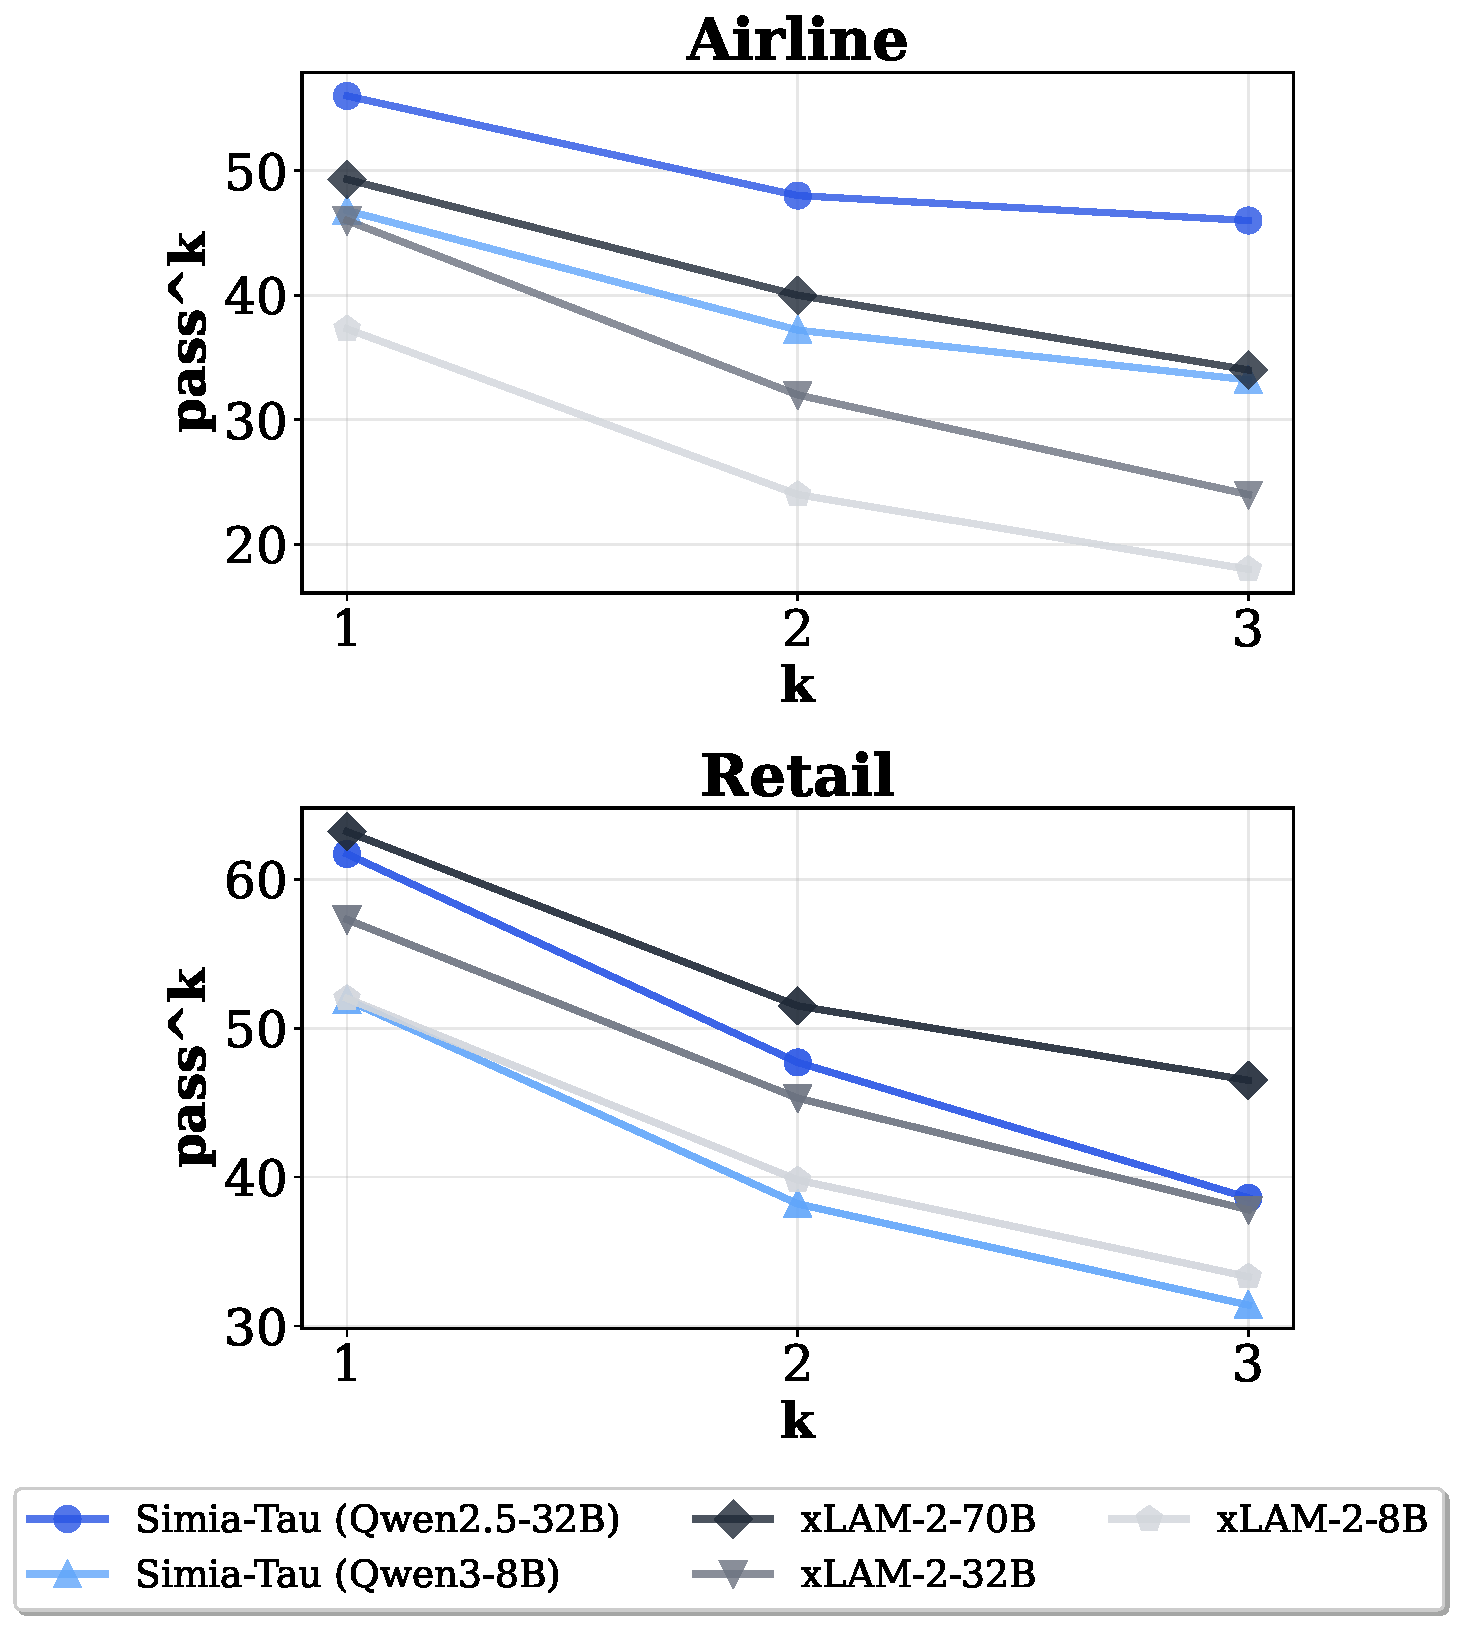
\includegraphics[width=0.9\linewidth]{figs/tau_bench_pass_power_k_comparison.pdf}

\caption{ \texttt{Pass\^{}k} performance comparison on the $\tau^2$-Bench across Airline and Retail domains for Simia-Tau and xLAM-2 models, with $k$ values of 1, 2, and 3. \texttt{Pass\^{}k} requires that each task should be successful for all the k retries, highlighting the robustness.}

  \label{fig:tau_bench_pass_power_k_comparison}
\end{figure}



\paragraph{Benchmarks.}
To assess the generality of our approach, we evaluate on three complementary agentic suites that span distinct domains and interaction types: (1) $\tau^2$-Bench (Airline, Retail)~\citep{barres2025tau}, a realistic tool-use benchmark emphasizing multi-turn API invocation, error recovery, and state tracking. Compared with $\tau$-Bench~\citep{yao2024tau}, $\tau^2$-Bench~\citep{barres2025tau} corrects potential erroneous tasks and enhances system implementation. Following \citep{barres2025tau}, we use GPT-4.1 as the user simulator (temperature set to 0) to generate user behaviors.
(2) OfficeBench~\citep{wang2024officebench} (2-apps, 3-apps), which evaluates cross-application workflows, compositional tool use, and coordination across office utilities.
(3) AgentBench~\citep{liu2023agentbench} (Operating System, WebShop, Mind2Web), which spans software manipulation, e-commerce goal completion, and open-web browsing.
Together, these suites comprehensively stress multi-step reasoning and tool-use competency across distinct domains.



\paragraph{Baselines.}
For reference, we report results from proprietary models including GPT-4, GPT-4o, GPT-4.1, o4-mini, and GPT-5. For open-source baselines, we fine-tune Qwen2.5-7B-Instruct and Qwen3-8B on the seed datasets of each suite; APIGen-MT (5k), AgentTuning (668), and OfficeBench 1-app tasks with o4-mini trajectories (76) using the same training recipe as our method. We further include the xLAM-2 model family~\citep{prabhakar2025apigen} and AgentLM family~\citep{zeng2023agenttuningenablinggeneralizedagent}, spanning model sizes from 1B to 70B.



\paragraph{RL Setup.} We implement RL experiments using RAGEN \citep{wang2025ragen} built on VeRL \citep{sheng2024hybridflow}. 
We conduct GRPO~\citep{shao2024deepseekmath} training followed by SFT under two configurations: (1) training on OfficeBench 1-app tasks and evaluating on OfficeBench 2-apps and 3-apps tasks, and (2) training on APIGen-MT-5k and evaluating on $\tau^2$-Bench airline and retail. We run GRPO training for 64 steps in both configurations. Detailed RL training hyperparameters are provided in Appendix~\ref{Grpo Setup}.


We utilize o4-mini to simulate the environment, which interacts with the model in each round, and computes the final reward. o4-mini is configured with a temperature of 1.0 and a maximum context length of 60,000 tokens. The complete tool usage specification, environment feedback format, the interaction history, and one reference sample trajectory are converted into text and incorporated into the o4-mini's prompt. 
Upon task completion or reaching the maximum number of interaction rounds, o4-mini will assess whether the task was successfully completed based on the trajectory. We assign a reward of 1 for successful task completion and 0 for failure. Detailed prompt are shown in Appendix \ref{appendix:prompt_rl}.


\subsection{Results}


\paragraph{$\tau^2$-bench.}
Table \ref{tab:taubench} shows that our Simia-Tau models demonstrate substantial performance gains across the Airline and Retail domains of the $\tau^2$-Bench. Notably, Simia-Tau (Qwen2.5-32B) achieves an average score of 58.9 (56.0 on Airline, 61.7 on Retail), outperforming GPT-4o by 4.7 points while trailing GPT-4.1 by only 0.2 points and o4-mini by 4.3 points. It also surpasses the baseline xLAM-2-32B (average 51.7) by 7.2 points and even exceeds xLAM-2-70B (average 56.3) by 2.6 points.



\definecolor{ourmodel}{RGB}{0, 0, 0}  % Black for our model
\definecolor{lightblue}{RGB}{220, 240, 255}  % Light blue background
\definecolor{gray}{RGB}{128, 128, 128}
\definecolor{lightgray}{RGB}{240, 240, 240}
\begin{table}
    \centering
    \caption{
        Performance on OfficeBench~\citep{wang2024officebench} across proprietary models, open baselines, and models fine-tuned on simulated trajectories. SFT followed by RL on simulated environments (\textbf{Simia-OB-RL}) also yields slight gains over SFT-only models (\textbf{Simia-OB}).
    }
    \label{tab:officebench_comparison}
    \resizebox{1\linewidth}{!}{
        \begin{tabular}{l|ccc}
            \toprule
            \textbf{Model} & \textbf{2-apps} & \textbf{3-apps} & \textbf{Average} \\
            \midrule
            \multicolumn{4}{c}{\textit{GPT Models}} \\
            \midrule
            GPT-5 & \underline{84.3} & \textbf{76.4} & \textbf{80.4} \\
            o4-mini & \textbf{86.3} & \underline{70.9} & \underline{78.6} \\
            GPT-4.1 & 78.4 & 63.6 & 71 \\
            GPT-4o & 74.5 & 50.9 & 62.7 \\
            GPT-4 & 50.6 & 11.6 & 31.1 \\
            \midrule
            \multicolumn{4}{c}{\textit{7B/8B Models}} \\
            \midrule
            \rowcolor{lightblue}
            \textbf{\textcolor{ourmodel}{Simia-OB-RL (Qwen2.5-7B)}} & \underline{64.7} & \textbf{34.5} & \underline{49.6} \\
            \rowcolor{lightblue}
            \textbf{\textcolor{ourmodel}{Simia-OB (Qwen3-8B)}} & 58.8 & \textbf{29.1} & \textbf{44.0} \\
            \addlinespace[3pt]
            \rowcolor{lightblue}
            \textbf{\textcolor{ourmodel}{Simia-OB (Qwen2.5-7B)}} & 57.8 & 27.3 & \underline{42.6} \\
            \rowcolor{lightblue}
            \textbf{\textcolor{ourmodel}{Simia-OB (Qwen2.5-Coder-7B)}} & \underline{64.7} & 14.6 & 39.7 \\
            \rowcolor{lightblue}
            \textbf{\textcolor{ourmodel}{Simia-OB (Llama-3.1-8B)}} & \textbf{64.9} & 12.7 & 33.8 \\
            Qwen3-8B-1apps-seed & 39.2 & 20 & 29.6 \\
            Qwen2.5-7B-Instruct-1apps-seed & 35.3 & 16.4 & 25.9 \\
            Qwen2.5-Coder-7B-Instruct & 31.4 & 10.7 & 21.1 \\
            Qwen2.5-7B-Instruct & 27.5 & 10.9 & 19.2 \\
            Llama-3.1-8B-Instruct & 7.8 & 3.6 & 5.7 \\
            Qwen3-$8B$ & 3.9 & 0 & 2.0 \\
            \midrule
            \multicolumn{4}{c}{\textit{3B Models}} \\
            \midrule
            \rowcolor{lightblue}
            \textbf{\textcolor{ourmodel}{Simia-OB (Qwen2.5-3B)}} & \textbf{43.1} & \textbf{9.1} & \textbf{26.1} \\
            \rowcolor{lightblue}
            \textbf{\textcolor{ourmodel}{Simia-OB (Llama-3.2-3B)}} & \textbf{43.1} & \underline{7.3} & \underline{25.2} \\
            Qwen2.5-3B-Instruct & \underline{15.7} & 1.8 & 8.8 \\
            Llama-3.2-3B-Instruct & 7.6 & 0 & 3.8 \\
            \midrule
            \multicolumn{4}{c}{\textit{1.5B Models}} \\
            \midrule
            \rowcolor{lightblue}
            \textbf{\textcolor{ourmodel}{Simia-OB (Qwen2.5-1.5B)}} & \textbf{33.3} & \textbf{5.5} & \textbf{19.4} \\
            Qwen2.5-1.5B-Instruct & \underline{5.9} & \underline{0} & \underline{3.0} \\
            \bottomrule
        \end{tabular}
    }
\end{table}




For 7B/8B-scale models, Simia-Tau (Qwen3-8B) attains an average score of 49.3 (46.7 on Airline, 51.9 on Retail), outperforming GPT-4 by 3.9 points and xLAM-2-8B (average 44.7) by 4.6 points. Furthermore, our Qwen3-8B substantially outperform models fine-tuned on APIGen-MT-5k, exceeding Qwen3-8B-APIGen-MT-5k (average 35.7) by 13.6 points. Additionally, after SFT and RL, Simia-tau-RL (Qwen-8B) achieves 49.0 and 52.9 on Ailine and Retail. 


Figure \ref{fig:tau_bench_pass_power_k_comparison} illustrates the \verb|Pass^k|~\citep{barres2025tau} performance of Simia-Tau and xLAM-2 models, evaluating the effect of varying $k$ values (1, 2, and 3) on task success rates. \verb|Pass^k|~\citep{barres2025tau} requires that each task should be successful for all the k retries to measure the robustness. Our Simia-Tau (Qwen2.5-32B) consistently achieves higher pass rates, with scores of 56.0, 48.0, and 46.0 for Airline, and 61.7, 47.7, and 38.6 for Retail, outperforming xLAM-2-70B Airline (49.3, 40.0, 34.0) and slightly less for Retail (63.2, 51.5, 46.5) as $k$ increases. 




\definecolor{ourmodel}{RGB}{0, 0, 0}  % Black for our model
\definecolor{lightblue}{RGB}{220, 240, 255}  % Light blue background
\definecolor{gray}{RGB}{128, 128, 128}
\definecolor{lightgray}{RGB}{240, 240, 240}
\begin{table}
    \centering
    \caption{
        Performance on Webshop, Mind2Web and Operating System~\citep{liu2023agentbench} across proprietary models, open baselines, and models fine-tuned on simulated trajectories.
        *GPT-4 results are reported from \citep{liu2023agentbench} and GPT-4o results are reported from leaderboard of SuperBench \citep{superbench_modeldetail}. 
    }
    \label{tab:agentbench_comparison}
    \resizebox{\linewidth}{!}{
        \begin{tabular}{l|ccc|c}
            \toprule
            \textbf{Model} & \textbf{Mind2Web} & \textbf{OS} & \textbf{Webshop} & \textbf{Average} \\
            \midrule
            \multicolumn{5}{c}{\textit{GPT Models}} \\
            \midrule
            GPT-4* & \underline{29} & \textbf{42.4} & \textbf{61.1} & \textbf{44.2} \\
            GPT-4o* & \textbf{32} & \underline{33.3} & \underline{48.9} & \underline{38.1} \\
            \midrule
            \multicolumn{5}{c}{\textit{$\geq$7B Models}} \\
            \midrule
            \rowcolor{lightblue}
            \textbf{\textcolor{ourmodel}{Simia-AB (Qwen3-8B)}} & \underline{25} & \textbf{34.5} & 67.3 & \textbf{42.6} \\
            \rowcolor{lightblue}
            \textbf{\textcolor{ourmodel}{Simia-AB (Qwen2.5-Coder-7B)}} & \textbf{29} & \underline{33} & 66 & \underline{42.6} \\
            \rowcolor{lightblue}
            \textbf{\textcolor{ourmodel}{Simia-AB (Qwen2.5-7B)}} & 23 & 32.6 & \underline{69.2} & 41.6 \\
            Qwen3-8B-seed & 22 & 31.3 & 68.6 & 40.6 \\
            Qwen2.5-7B-Instruct-seed & 12 & 29.1 & 68.2 & 36.4 \\
            AgentLM-70B & 13.5 & 21.5 & 64.9 & 33.3 \\
            Qwen3-8B & 21 & 27.8 & 49.5 & 32.8 \\
            AgentLM-13B & 8.4 & 18.1 & \textbf{70.8} & 32.4 \\
            Qwen2.5-7B-Instruct & 7 & 27.8 & 58.8 & 31.2 \\
            Llama-3.1-8B-Instruct & 18 & 19.4 & 54.9 & 30.8 \\
            Qwen2.5-Coder-7B-Instruct & 17 & 22 & 53 & 30.5 \\
            AgentLM-7B & 6.4 & 17.4 & 63.6 & 29.1 \\
            \midrule
            \multicolumn{5}{c}{\textit{3B Models}} \\
            \midrule
            \rowcolor{lightblue}
            \textbf{\textcolor{ourmodel}{Simia-AB (Llama-3.2-3B)}} & \textbf{26} & \underline{28} & \textbf{69} & \textbf{40.9} \\
            \rowcolor{lightblue}
            \textbf{\textcolor{ourmodel}{Simia-AB (Qwen2.5-3B)}} & \underline{23} & \textbf{31} & \underline{65} & \underline{39.9} \\
            Qwen2.5-3B-Instruct & 16 & 24 & 49 & 29.5 \\
            Llama-3.2-3B-Instruct & 15 & 17 & 49 & 27.0 \\
            \midrule
            \multicolumn{5}{c}{\textit{1.5B Models}} \\
            \midrule
            \rowcolor{lightblue}
            \textbf{\textcolor{ourmodel}{Simia-AB (Qwen2.5-1.5B)}} & \underline{17} & \textbf{15} & \textbf{54} & \textbf{28.5} \\
            Qwen2.5-1.5B-Instruct & \textbf{20} & \underline{13} & \underline{40} & \underline{24.0} \\
            \bottomrule
        \end{tabular}
    }
\end{table}

\paragraph{OfficeBench.}
Table~\ref{tab:officebench_comparison} shows that our Simia-OB models demonstrate substantial improvements in office automation tasks on the OfficeBench, which evaluates language agents' ability to handle complex workflows involving multiple applications such as Word, Excel, calendars, and emails. Notably, Simia-OB (Qwen3-8B) achieves an average score of 44.0 (58.8 on 2-apps, 29.1 on 3-apps), outperforming GPT-4 (average 31.1) by 12.9 points. Other variants, such as Simia-OB (Qwen2.5-7B) with 42.6 average and Simia-OB (Qwen2.5-Coder-7B) with 39.7, further highlight the efficacy of our approach in bridging the gap between small models and proprietary giants. For the Qwen3-8B model, the $\text{thinking}$ behavior leads to excessively long CoT sequences and repetitive patterns, which results in performance scores approaching zero. 

Compared with the model fine-tuned on the seed data with real environments, Simia-OB (Qwen3-8B)  outperforms baselines Qwen3-8B-1apps-seed (average 29.6) by 14.4 points. Similarly, Simia-OB (Qwen2.5-7B) exceeds Qwen2.5-7B-Instruct-1apps-seed (average 25.9) by 16.7 points. 



\begin{figure*}
    \centering
    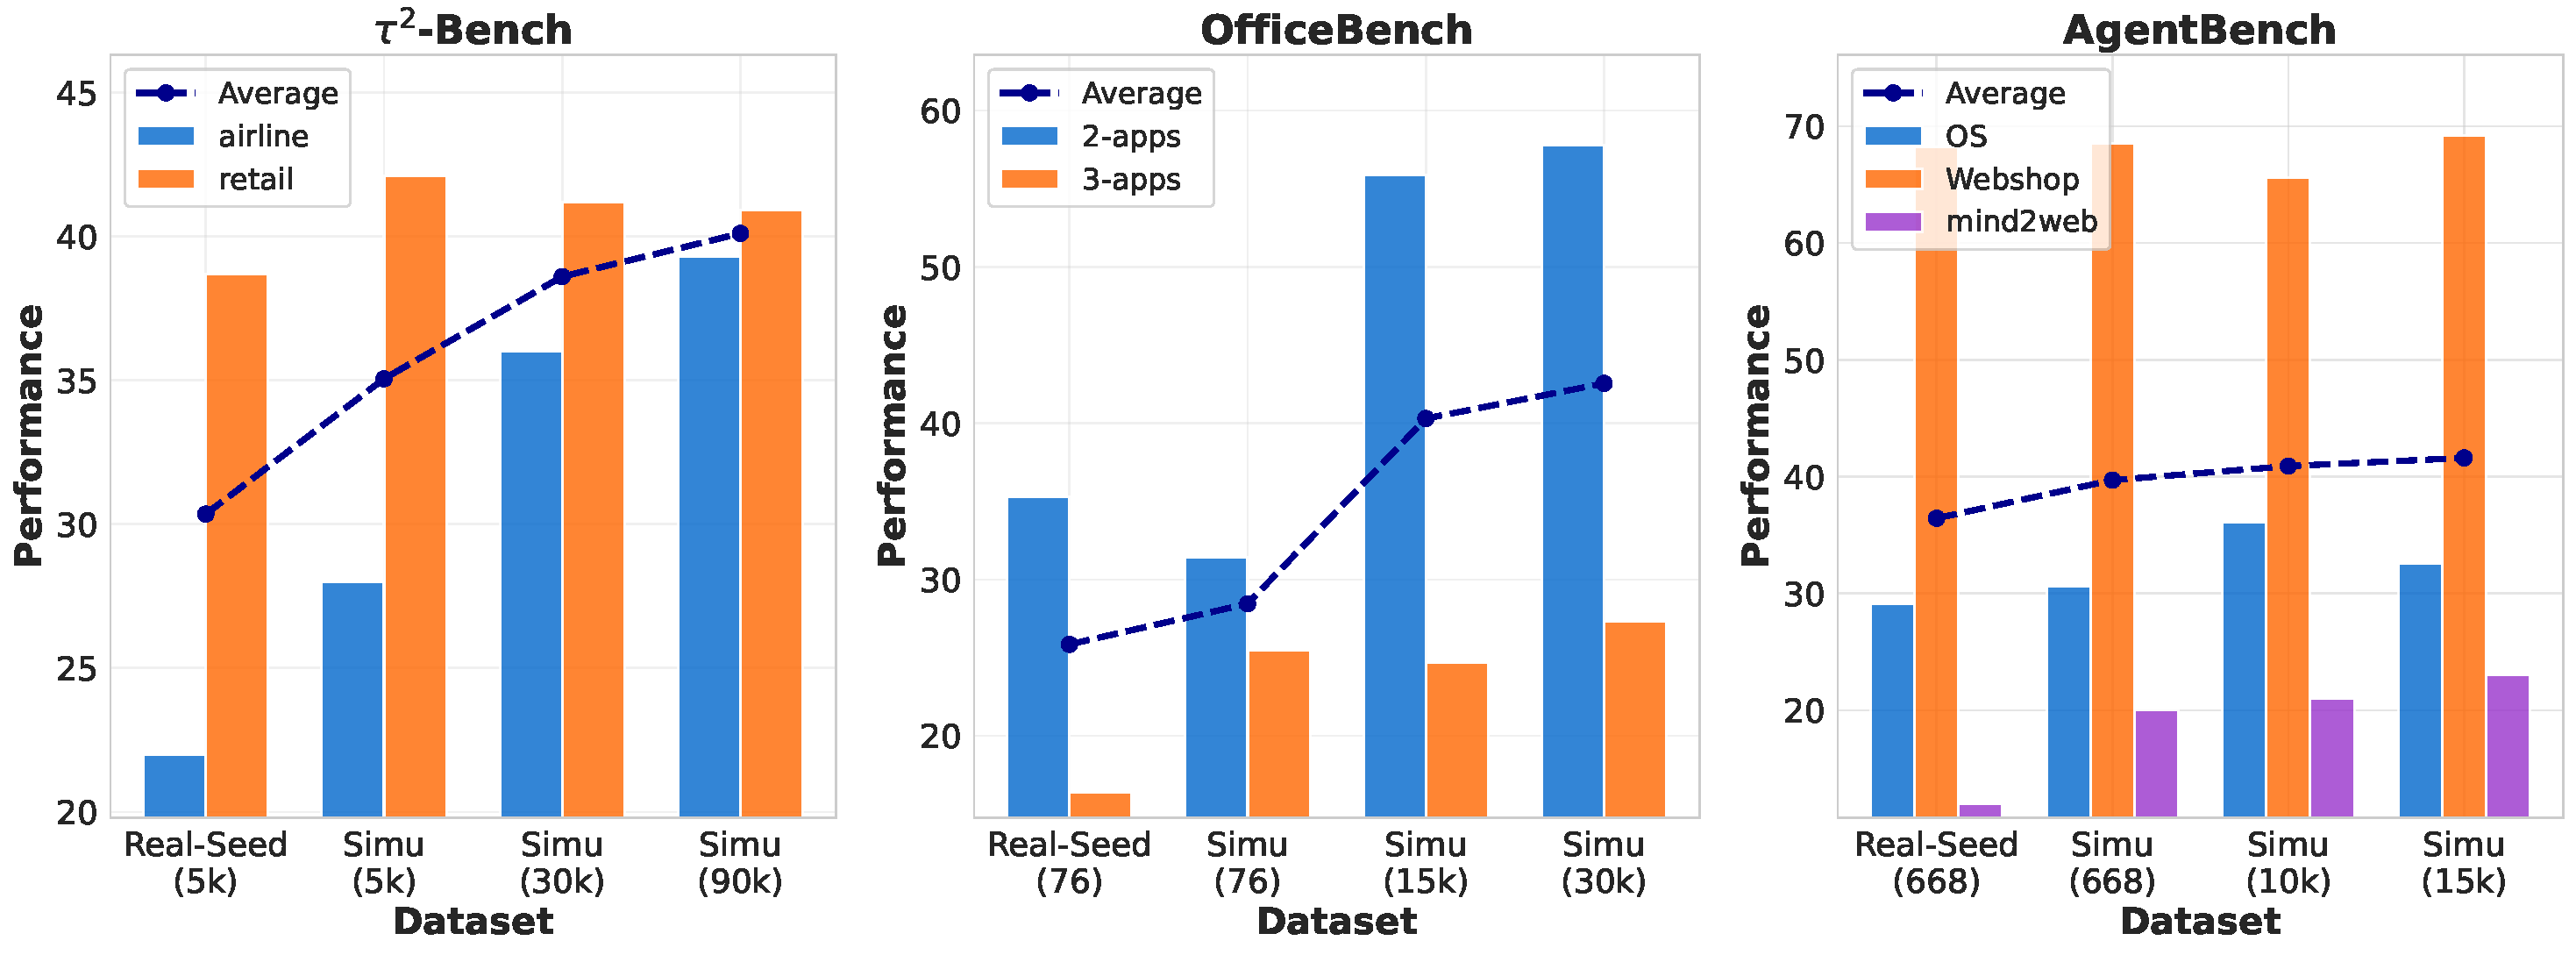
\includegraphics[width=\textwidth]{figs/ablation_on_datasize.pdf}
    \caption{Ablation study on dataset generated by real environment and simulated environment. When the dataset size is identical, we show that simulated trajectories achieve performance comparable to real-environment-based trajectories on OfficeBench and AgentBench, and even better on $\tau^2$-bench. As dataset size scales, simulated trajectories significantly improve model performance. This highlights the potential of simulated environments to support larger, more diverse datasets, addressing the limitations of real-world seed data constrained by collection efforts. }
    \label{fig:ablation_on_datasize}
\end{figure*}

\paragraph{AgentBench.} Our models exhibit competitive performance across Mind2Web, Operating System (OS), and Webshop, as presented in Table~\ref{tab:agentbench_comparison}. Our Simia-AB (Qwen3-8B) achieves an average score of 42.6, with a standout 34.5 on OS and 67.3 on Webshop, closely matching GPT-4’s 44.2 average and surpassing GPT-4o’s 38.1. The Simia-AB (Qwen2.5-Coder-7B) model ties with Qwen3-8B at 42.6 average, excelling with 29 on Mind2Web and 66 on Webshop, though it lags slightly on OS (33). The Qwen2.5-7B model leads with a Webshop score of 69.2, outperforming GPT-4 (61.1) and GPT-4o (48.9), with an overall average of 41.6. Both of our fine-tuned Qwen3-8B and Qwen2.5-7B-instruct models are better than their variants finetuned on the seed dataset generated from real environment. 







\begin{figure*}
  \centering
  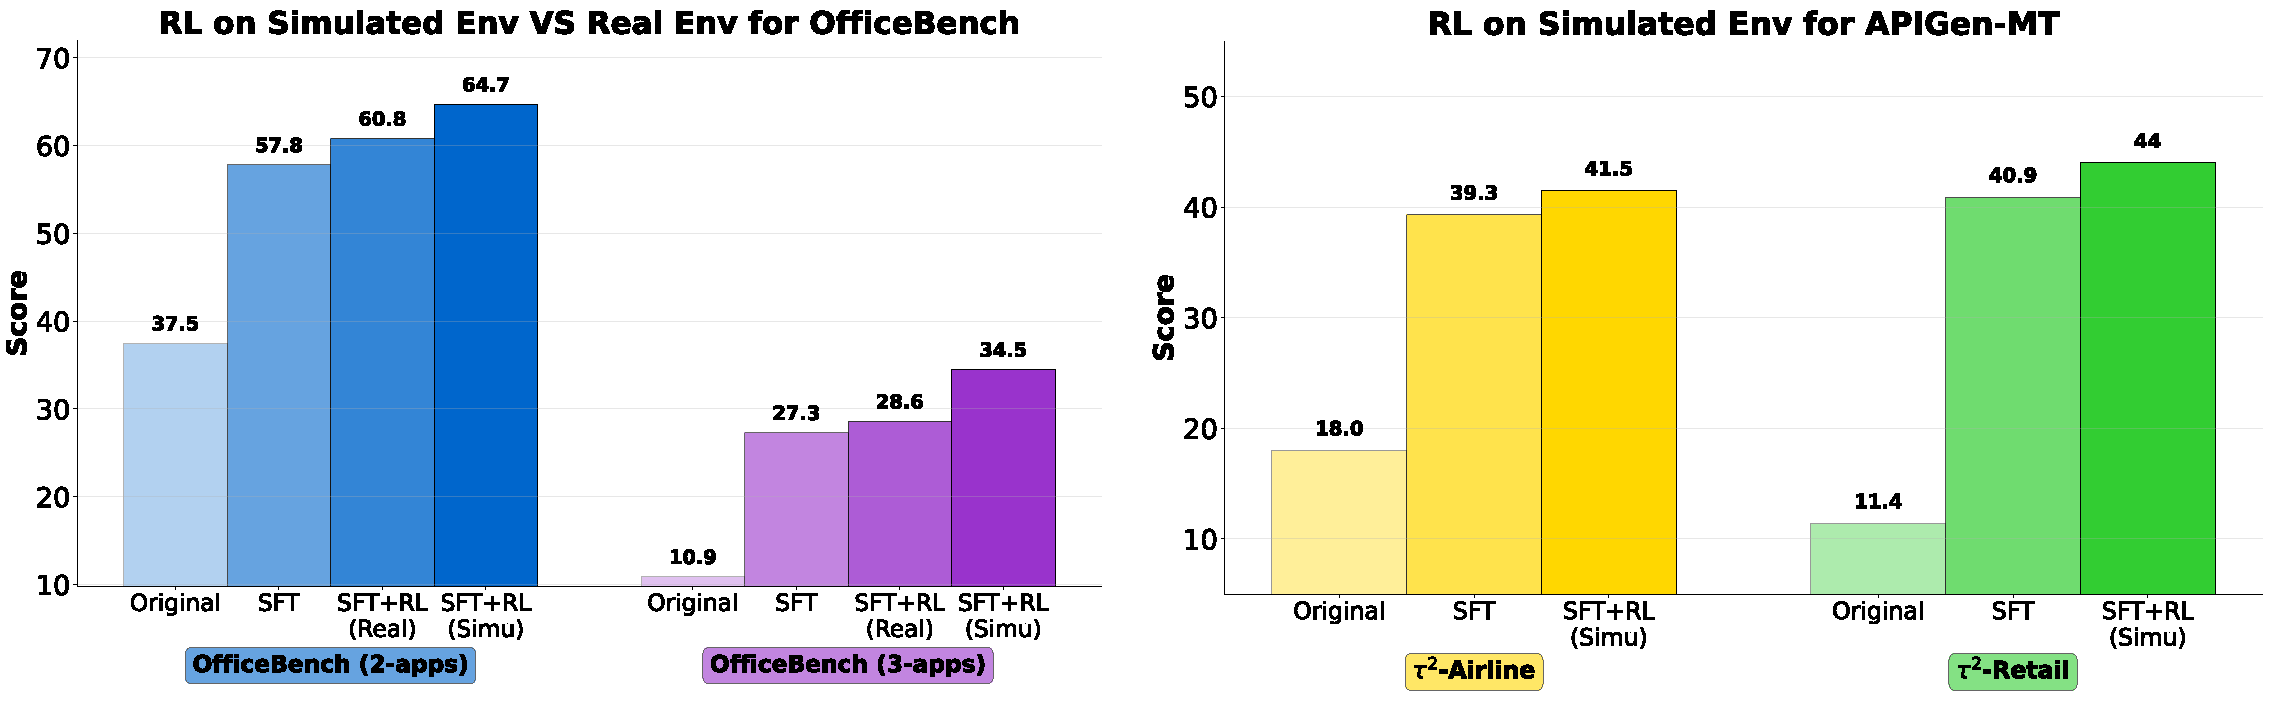
\includegraphics[width=\textwidth]{figs/rl_agent_training_diagram_rl_1015-3_cropped.pdf}
  \caption{RL on simulated environment followed by SFT for Qwen2.5-7B-Instruct model.}
  \label{fig:sft_rl_officebench}
\end{figure*}


\paragraph{Trajectory by Real Env V.S. Simulated Env.} Figure \ref{fig:ablation_on_datasize} shows the performance of Qwen2.5-7B-Instruct fine-tuned on trajectories generated from real environment (seed dataset) and simulated environments (our synthesized dataset). When trained on datasets of identical size (e.g., for $\tau^2$-bench we compare the model fine-tuned on 5k seed data and 5k synthesized data), we find that synthesized trajectories achieve performance comparable to real-environment-based trajectories on OfficeBench and AgentBench, even better on $\tau^2$-bench. As dataset size expands, synthesized trajectories significantly outperform seed-based ones, demonstrating the scalability advantage of synthesized data with simulated environments. This highlights the potential of simulated environments to support larger, more diverse datasets, addressing the limitations of real-world seed data constrained by collection efforts.



\begin{figure*}
    \centering
    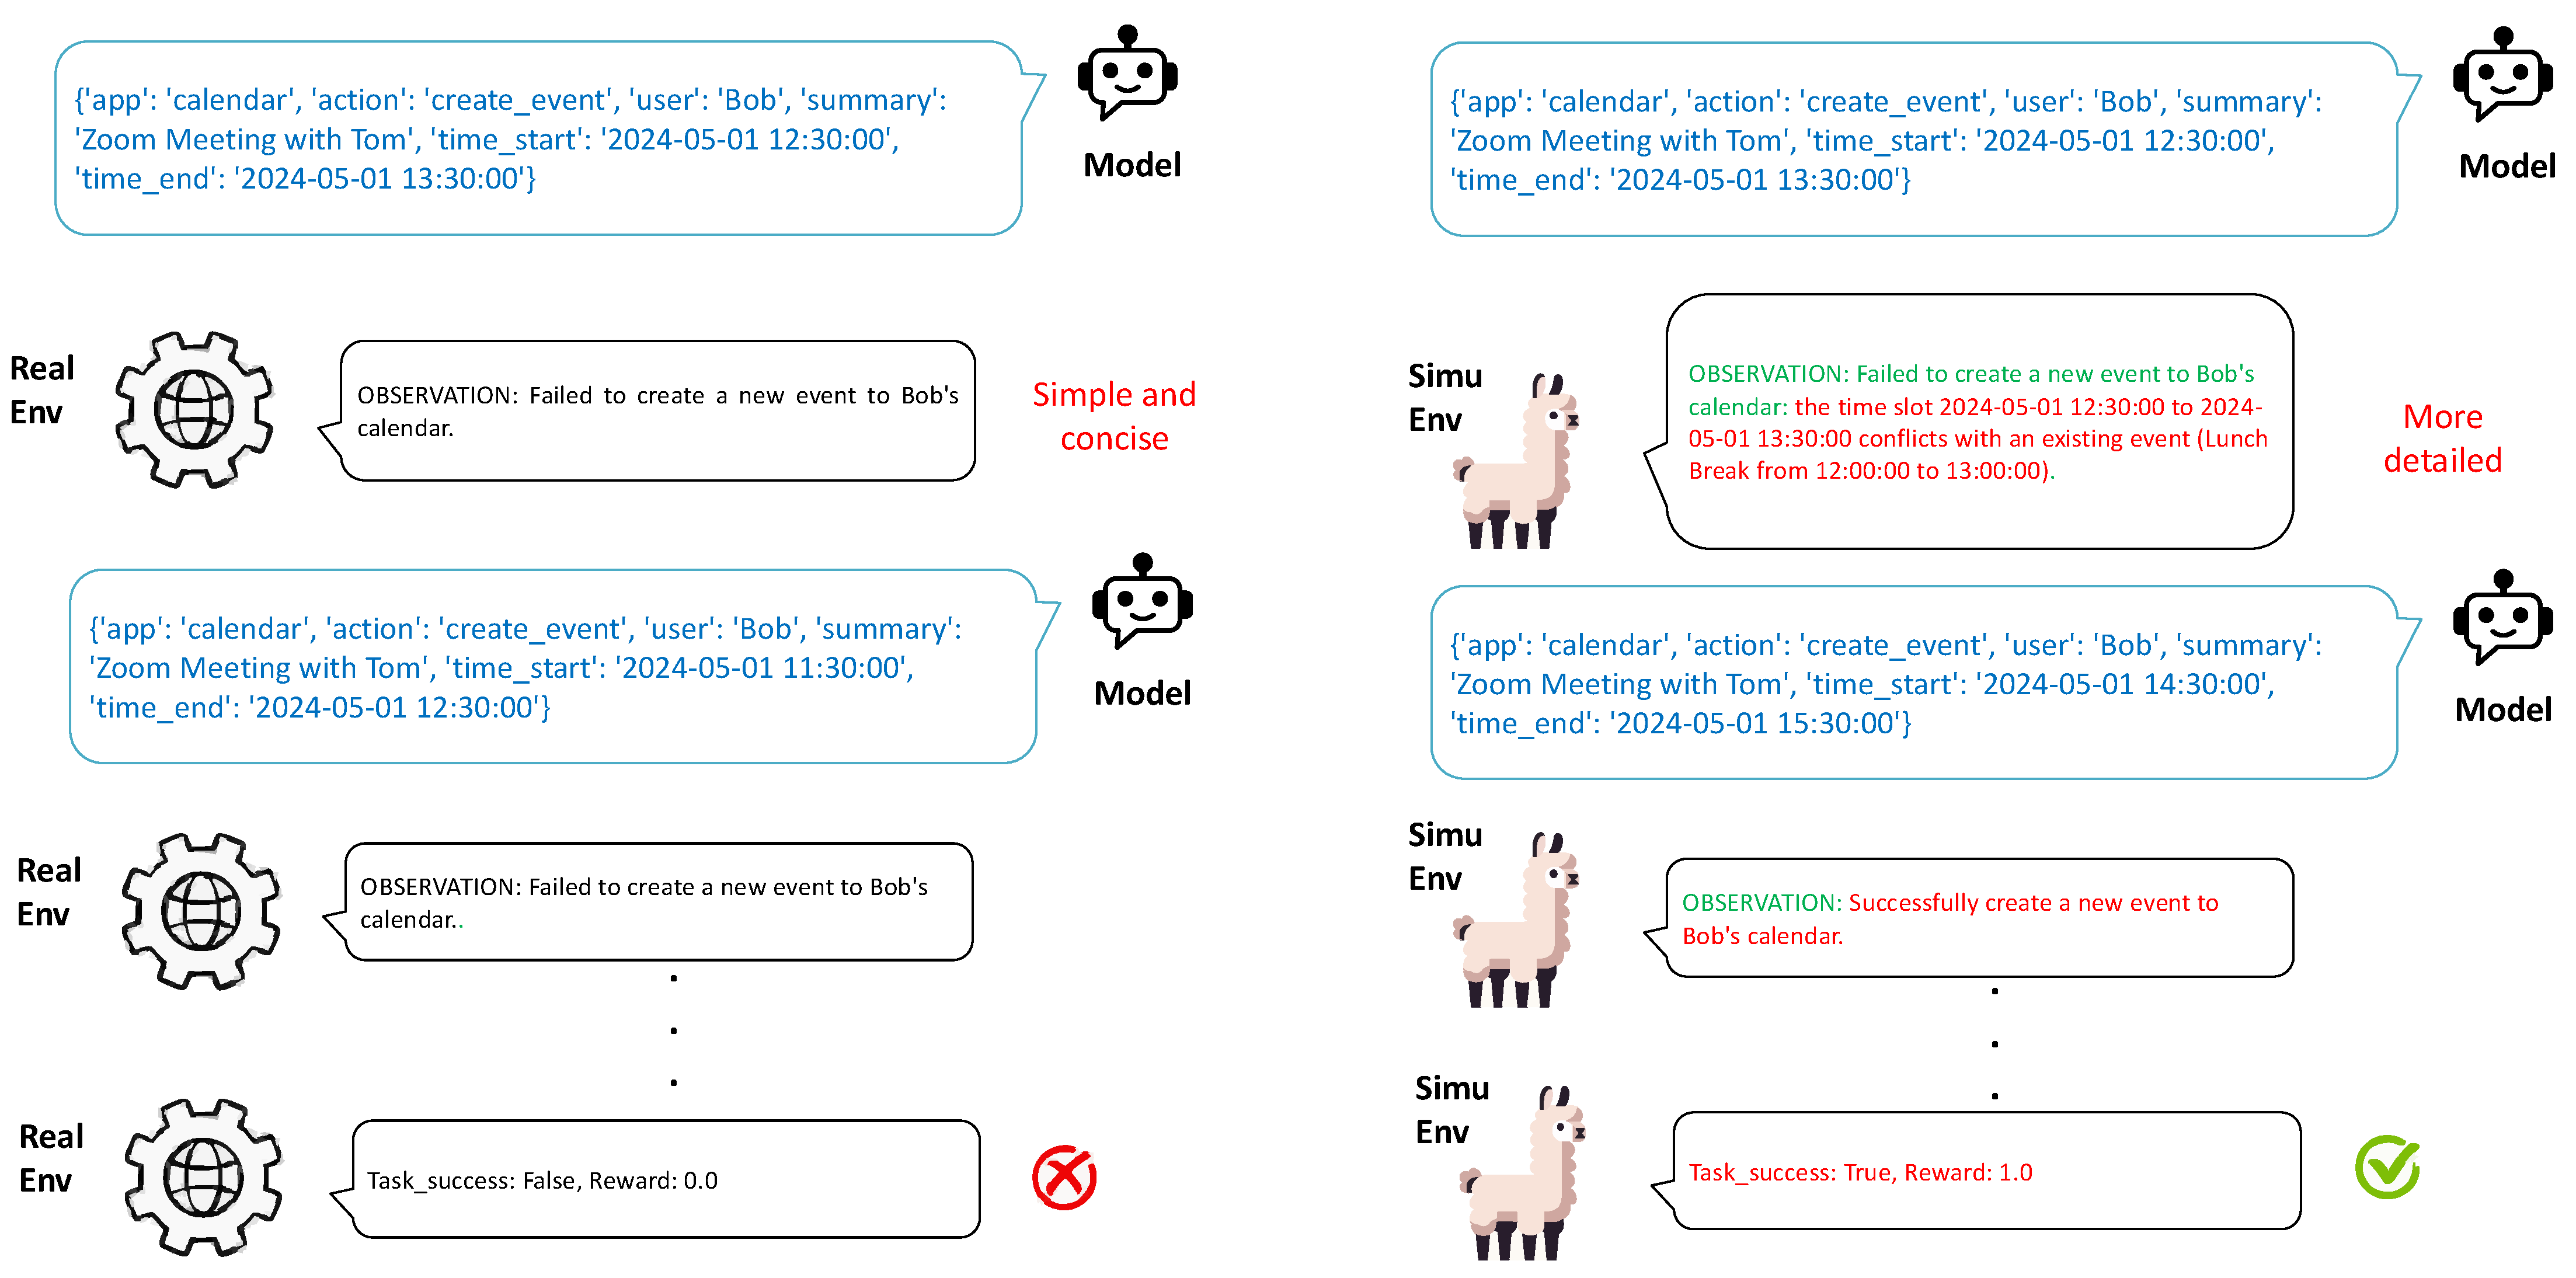
\includegraphics[width=0.9\textwidth]{figs/rl_case_study.pdf}
    \caption{Case study comparing RL on real and simulated environments.
In the real setting (left), the system displays only the fixed failure messages inherently provided by the original environment \cite{wang2024officebench}. In contrast, the simulated environment (right) generates more flexible and detailed feedback, explaining conflicts (e.g., overlapping with a lunch break) and enabling the model to adjust and eventually get the reward.}
    \label{fig:rl_case_study}
\end{figure*}



\subsection{RL Results}
\paragraph{Results of RL on Simulated Env.} Figure \ref{fig:sft_rl_officebench} demonstrates the results of RL on simulated environments for Qwen2.5-7B-Instruct. For OfficeBench, We observe that the simulated environment (64.7, 34.5) outperforms the real environment (60.8 28.6) on OfficeBench 2-apps and 3-apps, yielding total improvements of 6.9 and 7.2 points over the model after SFT. On $\tau^2$-Bench, SFT followed by RL yields slight additional gains. Note that $\tau^2$-Bench real environment requires simulated users for dynamic agent interaction, we do not directly compare simulated and real environments for $\tau^2$-Bench. 


In the real setting (left), the system displays only the fixed and concise failure messages inherently provided by the original environment.

\paragraph{Case Study of RL on Simulated Env for OfficeBench.} 
We present in Figure \ref{fig:rl_case_study} a case study highlighting how RL surprisingly benefits more from the simulated environment than from the real one. In the real setting (left), the system displays only the fixed and concise failure messages inherently provided by the original environment \cite{wang2024officebench}. By contrast, the simulated environment (right) offers richer and more adaptive feedback, e.g., pointing out conflicts such as overlapping with a lunch break, which helps the model adjust its behavior and ultimately achieve the reward. 




\subsection{More Ablations}
\paragraph{Ablation on Different Trajectory Simulators.}
We compare performances of different trajectory simulators in Appendix \ref{More Results of Synthetic Data}.

\paragraph{Training on Combined Datasets.}
We train Qwen3-8B on combined three datasets jointly. See more details in Appendix~\ref{More Results of Synthetic Data}.

